\subsection{Complex Functions}
\subsubsection{Mapping Properties of Simple Functions}
Similar to how functions with real variables map values to a different set of values, complex functions do the same. The main difference is that with complex functions we're mapping a 2 dimensional set of inputs to a 2 dimensional set of outputs.
\[
w=f(z)=u+iv
\]
We define $z\in \mathcal{S}$ the image of $\mathcal{S}$ under $w$.\\
Some common mappings:
\begin{itemize}
    \item The identity map
    \begin{align*}
        &w=f(z)=z\\
        &\eqnsystem{u=x\\ v=y}
    \end{align*}
    \item Translation by $z_0$
    \begin{align*}
        &w=f(z)=z+z_0\\
        &\eqnsystem{u=x+x_0\\ v=y+y_0}
    \end{align*}
    \item Stretching ($a>1$) or contraction ($a<1$)
    \begin{align*}
        &w=f(z)=az=are^{i\varphi},\ a\in\R\\
        &\eqnsystem{u=ax\\ v=ay}
    \end{align*}
    \item Rotation by $\varphi_0$
    \begin{align*}
        &w=f(z)=e^{i\varphi_0}z=e^{i(\varphi+\varphi_0)}
    \end{align*}
\end{itemize}
Using these basic mapping principles we are able to lay the foundation for some more complicated mappings.\\
Ex: Find the image of $S=\brcurly{|z-1|\geq1}$ under the mapping $f(z)=\frac{1}{z}$\\
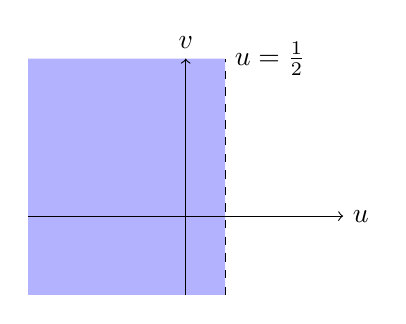
\begin{tikzpicture}
    % Region u <= 1/2
    \fill[blue!30, domain=-2:0.5, variable=\x]
        (-2, -1) -- plot ({\x}, {2}) -- (0.5, -1) -- cycle;

    % Axes
    \draw[->] (-2,0) -- (2,0) node[right] {$u$};
    \draw[->] (0,-1) -- (0,2) node[above] {$v$};
    
    % Dashed line u = 1/2
    \draw[dashed] (0.5, -1) -- (0.5, 2) node[right] {$u=\frac{1}{2}$};
\end{tikzpicture}

\begin{align*}
    &z=\frac{1}{w}=\frac{1}{u+iv}=\frac{u-iv}{u^2+v^2}\\
    &x=\frac{u}{u^2+v^2}\\
    &y=-\frac{v}{u^2+v^2}\\
    &|z-1|\geq1\Ra\brvertical{\frac{1}{w}-1}\geq1\\
    &\frac{1-w}{w}\geq1\\
    &|1-w|\geq|w|\\
    &|1-w|^2\geq|w|^2\\
    &(1-u)^2+v^2\geq u^2+v^2\\
    &-2u+1\geq 0\\
    &u\leq\frac{1}{2}\\
    &S'=\brcurly{u\leq\frac{1}{2}}
\end{align*}


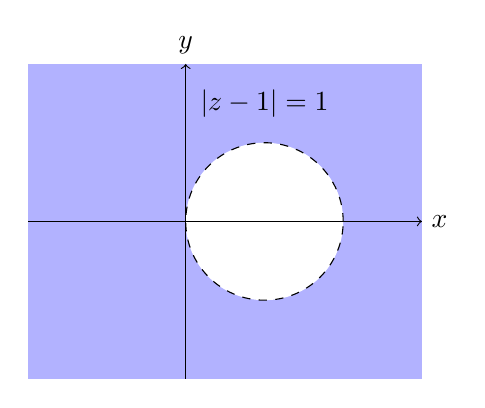
\begin{tikzpicture}
    % Background (Blue)
    \fill[blue!30] (-2,-2) rectangle (3,2);

    % Region |z-1| >= 1
    \fill[blue!30, domain=-1:1, variable=\x]
        (-2, 0) -- plot ({1+\x}, {sqrt(1 - \x*\x)}) -- (2, 0) -- cycle;
    \fill[blue!30, domain=-1:1, variable=\x]
        (-2, 0) -- plot ({1+\x}, {-sqrt(1 - \x*\x)}) -- (2, 0) -- cycle;

    % Circle (White, Dashed)
    \draw[fill=white, dashed] (1, 0) circle (1);

    % Label: |z-1| = 1
    \node at (1, 1.5) {$|z-1|=1$};

    % Axes
    \draw[->] (-2,0) -- (3,0) node[right] {$x$};
    \draw[->] (0,-2) -- (0,2) node[above] {$y$};
\end{tikzpicture}

Ex2: Find the image of $S=\brcurly{x\leq1}$ under the mapping $f(z)=\frac{1}{z}$

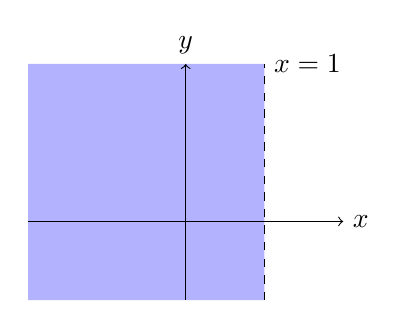
\begin{tikzpicture}
    % Region x <= 1
    \fill[blue!30, domain=-2:1, variable=\x]
        (-2, -1) -- plot ({\x}, {2}) -- (1, -1) -- cycle;

    % Axes
    \draw[->] (-2,0) -- (2,0) node[right] {$x$};
    \draw[->] (0,-1) -- (0,2) node[above] {$y$};
    
    % Dashed line x = 1
    \draw[dashed] (1, -1) -- (1, 2) node[right] {$x=1$};
\end{tikzpicture}
\begin{align*}
    &z=\frac{1}{w}=\frac{1}{u+iv}=\frac{u-iv}{u^2+v^2}\\
    &x=\frac{u}{u^2+v^2}\\
    &x\leq1\Ra \frac{u}{u^2+v^2}\leq1\Ra u^2+v^2\geq u\\
    &(u-\tfrac{1}{2})^2+v^2\geq\tfrac{1}{4}
\end{align*}

% create a new tikzpicture of the circle |z-\frac{1}{2}|>=1/2
\begin{tikzpicture}
    % Background (Blue)
    \fill[blue!30] (-2,-2) rectangle (3,2);

    % Region |z-1| >= 1
    \fill[blue!30, domain=-1:1, variable=\x]
        (-2, 0) -- plot ({1+\x}, {sqrt(1 - \x*\x)}) -- (2, 0) -- cycle;
    \fill[blue!30, domain=-1:1, variable=\x]
        (-2, 0) -- plot ({1+\x}, {-sqrt(1 - \x*\x)}) -- (2, 0) -- cycle;

    % Circle (White, Dashed)
    \draw[fill=white, dashed] (1, 0) circle (1);

    % Label: |z-1| = 1
    \node at (1, 1.5) {$|z-\tfrac{1}{2}|=\tfrac{1}{2}$};

    % Axes
    \draw[->] (-2,0) -- (3,0) node[right] {$x$};
    \draw[->] (0,-2) -- (0,2) node[above] {$y$};
\end{tikzpicture}\\
We see from the previous two examples that circles map to lines and lines map to circles. Let's see why this is the case.
\begin{align*}
    &a(x^2+y^2)+bx+cy+d=0\\
    &a|z|^2+b\frac{z+\bar{z}}{2}+c\frac{z-\bar{z}}{2i}+d=0
\end{align*}
In the case where $a=0$, we have a line. In the case where $a\neq0$, we have a circle.
\begin{align*}
    &w=\frac{1}{z}\Ra z=\frac{1}{w}\\
    &z\bar{z}=|z|^2=\frac{1}{|w|^2}=\frac{1}{w\bar{w}}\\
    &a\frac{1}{w\bar{w}}+b\frac{z+\bar{z}}{2}+c\frac{z-\bar{z}}{2i}+d=0\\
    &a\frac{1}{w\bar{w}}+\frac{b}{2}\brround{\frac{1}{w}+\frac{1}{\bar{w}}}+\frac{c}{2i}\brround{\frac{1}{w}-\frac{1}{\bar{w}}}+d=0\\
    &a+\frac{b}{2}\brround{w+\bar{w}}+\frac{c}{2i}\brround{w-\bar{w}}+d\brround{w\bar{w}}=0\\
\end{align*}
If we have a linear transformation of the form $az+b$ it corresponds to the scaling and translation of the set only. A line will map to a line and a circle will map to a circle.\\
We can combine this with the $w=\frac{1}{z}$ transformation property to get a more general transformation. We call this the \textit{Mobius transformation}:
$$f(z)=\frac{az+b}{cz+d}=\frac{a}{c}+\frac{b-\tfrac{ad}{c}}{cz+d}$$
where $a,b,c,d\in\C$

Ex: Find the mapping of $f(z)=\frac{1}{z+1}$ on the set $S=\brcurly{\Re(z)>0}$ 
\begin{align*}
    &u+iv=\frac{1}{x+1+iy}\Ra x+1+iy=\frac{1}{u+iv}\\
    &x+1=\frac{u}{u^2+v^2}\\
    &x>0\Ra x+1>1\\
    &\frac{u}{u^2+v^2}>1\Ra u>u^2+v^2\\
    &u^2+v^2-u+\frac{1}{4}<\frac{1}{4}\\
    &\brround{u-\frac{1}{2}}^2+v^2<\frac{1}{4}\\
    &S'=\brcurly{w=u+iv\Bigg\vert\brround{u-\frac{1}{2}}^2+v^2<\bfrac{1}{2}^2}
\end{align*}

Ex2: Find the mapping of $f(z)=\frac{z-i}{z+i}$ on $S=\brcurly{|z|<3}$
\begin{align*}
    &wz+iw=z-i\Ra z(w-1)=-i-iw\Ra z=\frac{i(w+1)}{1-w}\\
    &|z|=\frac{|w+1|}{|w-1|}<3\\
    &|w+1|<3|w-1|\Ra |w+1|^2<9|w-1|^2\\
    &(u+1)^2+v^2<9(u-1)^2+9v^2\\
    &u^2+2u+1+v^2<9u^2-18u+9+9v^2\\
    &0<8u^2-20u+8+8v^2\Ra 0<u^2-\frac{5}{2}u+1+v^2\\
    &\frac{9}{16}<u^2-\frac{5}{2}u+\frac{25}{16}+v^2\\
    &\frac{9}{16}<\brround{u-\frac{5}{4}}^2+v^2\\
    &S'=\brcurly{w=u+iv\Bigg\vert\brround{u-\frac{5}{4}}^2+v^2>\bfrac{3}{4}^2}
\end{align*}

Another common mapping is the $f(z)=z^2$ or more generally $f(z)=z^n$ mapping.
For $w=z^2$,
\[w=z^2=r^2e^{2i\varphi}\Ra \eqnsystem{|w|=|z|^2\\ \arg(w)=2\arg(z)}\]
This mapping scales the magnitude but more notably, it doubles the argument. This means that the mapping of a half circle will now be a full circle.\\

Ex: Find the mapping of $f(z)=z^2$ on $S=\brcurly{0\leq \Re(z)\leq1,\Im(z)=1}$
\begin{align*}
    &w=x^2+i2xy-y^2\\
    &u=x^2-y^2=x^2-1\Ra -1\leq u\leq 0\\
    &v=2xy=2x\Ra 0\leq v\leq 2\\
    &S'=\brcurly{w=u+iv|-1\leq u\leq 0,\ 0\leq v\leq 2}
\end{align*}
Ex2: Find the mapping of $f(z)=-2z^5$ on $S=\brcurly{|z|<1,0<\Arg(z)<\frac{\pi}{2}}$
\begin{align*}
    &z^5=-\frac{w}{2}\Ra |z|^5=\frac{|w|}{2}<1\Ra |w|<2\\
    &5\arg(z)=\arg(w)\pm\pi \\
    &0<\arg(w)\pm\pi <\frac{5\pi}{2}\\
    &-\pi<\arg(w)<\frac{3\pi}{2}\\
    &S'=\brcurly{|w|<2}
\end{align*}

Another common mapping is the $f(z)=e^z$ mapping.
\begin{align*}
    &w=e^z=e^{x+iy}=e^xe^{iy}\\
    &\eqnsystem{|w|=e^x\\ \arg(w)=y}
\end{align*}
\centerline{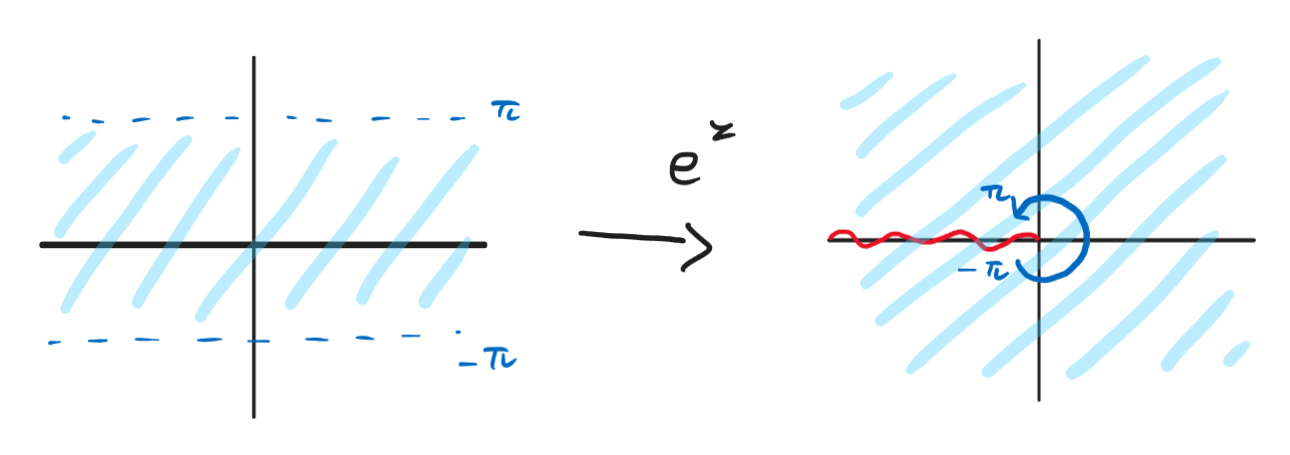
\includegraphics[width=0.8\textwidth]{Images/ComplexAnalysisPictures/ExponentialMapping.png}}\\
This mapping has the property that the magnitude is only dependent on $x$ and the argument is exactly $y$.\\
Ex: Find the mapping of $f(z)=e^z$ on $S=\brcurly{\Re(z)=1}$
\begin{align*}
    &w=e^xe^{iy}\\
    &|w|=e,\ \arg(w)=y\\
    &S'=\brcurly{|w|=e}
\end{align*}
Ex2: Find the mapping of $f(z)=e^z$ on $S=\brcurly{0\leq \Im(z)\leq\frac{\pi}{4}}$
\begin{align*}
    &|w|=x\\
    &\arg(w)=y\Ra 0\leq \arg(w)\leq \frac{\pi}{4}\\
    &S'=\brcurly{0\leq \Arg(w)\leq \frac{\pi}{4}}
\end{align*}
Ex3: Find the mapping of $f(z)=e^{iz}$ on $S=\brcurly{z: -\frac{\pi}{2}\leq \Re(z)\leq \pi,-1\leq\Im(z)\leq1}$\\
(Note that multiplying $z$ by $i$ rotates it by $90^\circ$)
\begin{align*}
    &w=e^{iz}=e^{ix}e^{-y}\\
    &|w|=e^{-y}\Ra e^{-1}\leq|w|\leq e\\
    &\arg(w)=x\Ra -\frac{\pi}{2}\leq \arg(w)\leq\pi\\
    &S'=\brcurly{w\Bigg\vert e^{-1}\leq|w|\leq e,-\frac{\pi}{2}\leq \arg(w)\leq\pi}
\end{align*}
Ex4: Prove 
\[ |e^{-z^3}|\leq 1\ \forall \brcurly{z\Bigg\vert-\frac{\pi}{6}\leq\Arg(z)\leq\frac{\pi}{6}} \]
\begin{proof}
We can express $-z^3$ as some complex number $a+ib$ where $a=\Re(-z^3)$ and $b=\Im(-z^3)$. Taking the magnitude gives
\[ |e^{-z^3}|=|e^{a+ib}|=|e^ae^{ib}|=|e^a||e^{ib}|=|e^a|=|e^{\Re(-z^3)}| \]
$z$ can be written as
\begin{align*}
    &z=|z|e^{i\Arg(z)}\\
    &z^3=|z|^3e^{i3\Arg(z)}=|z|^3\brround{\cos(3\Arg(z))+i\sin(3\Arg(z))}\\
    &-z^3=-|z|^3\brround{\cos(3\Arg(z))+i\sin(3\Arg(z))}\\
    &\Re(-z^3)=-|z|^3\cos(3\Arg(z))\\
    &\Arg(z)\in\brsquare{-\frac{\pi}{6},\frac{\pi}{6}}\\
    &\Ra 3\Arg(z)\in\brsquare{-\frac{\pi}{2},\frac{\pi}{2}}\\
    &\cos(3\Arg(z))\in\brsquare{0,1}\\
    &|z|^3\in\brcurly{x\in\R|x\geq0}\\
    &\Re(-z^3)=-|z|^3\cos(3\Arg(z))\in\brcurly{x\in\R|x\leq0}\\
    &e^{\Re(-z^3)}\in[0,1]\\
    &\Ra |e^{-z^3}|\leq1
\end{align*}
\end{proof}

\subsubsection{Calculus of Complex Functions}
We define the limit of a complex function to be
\begin{align*}
    &w=f(z)=u+iv\\
    &\lim_{z\to z_0}f(z)=\lim_{(x,y)\to(x_0,y_0)}u(x,y)+i\lim_{(x,y)\to(x_0,y_0)}v(x,y)
\end{align*}
Note that the notation $(x,y)\to(x_0,y_0)$ means that the limit is taken as $(x,y)$ approaches $(x_0,y_0)$ along \textit{any} path.\\
The usual limit arithmetic rules are able to be applied as with real numbers.\\
In order for
$\lim\limits_{z\to z_0}f(z)$
to exist, we require that both $\lim\limits_{(x,y)\to(x_0,y_0)}u(x,y)$ and $\lim\limits_{(x,y)\to(x_0,y_0)}v(x,y)$ exist.\\
If we define $z_0=x_0+iy_0$ then we can define the derivative of a complex function as
$$f'(z_0)=\lim_{z\to z_0}\frac{f(z)-f(z_0)}{z-z_0}=\lim_{\Delta z\to0}\frac{f(z_0+\Delta z)-f(z_0)}{\Delta z}$$
If this limit exists then the function is said to be differentiable at $z_0$.\\
Ex: $f(z)=z$
\begin{align*}
    &f'(z_0)=\lim_{\Delta z\to0}\frac{f(z_0+\Delta z)-f(z_0)}{\Delta z}=\frac{z_0+\Delta z-z_0}{\Delta z}=1\\
    &\Ra f'(z_0)=1
\end{align*}
Ex2: $f(z)=\bar{z}$
\begin{align*}
    &f'(z)=\lim_{\Delta z\to0}\frac{f(z+\Delta z)-f(z)}{\Delta z}=\lim_{\Delta z\to0}\frac{\overline{\Delta z}}{\Delta z}\\
    &\Delta z=h_1+ih_2\Ra \overline{\Delta z}=h_1-ih_2\\
    &h_2=0:\ \lim_{\Delta z\to0}\frac{\overline{\Delta z}}{\Delta z}=\lim_{h_1\to0}\frac{h_1}{h_1}=1\\
    &h_1=0:\ \lim_{\Delta z\to0}\frac{\overline{\Delta z}}{\Delta z}=\lim_{h_2\to0}\frac{-ih_2}{ih_2}=-1\\
    &\lim_{h_1\to0}\frac{h_1}{h_1}\neq\lim_{h_2\to0}\frac{-ih_2}{ih_2}\ \therefore\text{ the derivative does not exist}
\end{align*}
An easy way to determine if a function is differentiable is to use the Cauchy-Riemann equations.\\
Any path that can be taken to approach $z_0$ can be written as a linear combination of the paths $\Delta z=\Delta x$ and $\Delta z = i\Delta y$ so the derivative must satisfy both of these paths.
\begin{align*}
    &f'(z_0)=\lim_{\Delta z\to0}\frac{f(z_0+\Delta z)-f(z_0)}{\Delta z}\\
    &f(z_0)=u(x_0,y_0)+iv(x_0,y_0)\\
    &\text{Define }\Delta z=\Delta x\\
    &f'(z_0)=\lim_{\Delta x\to 0}\frac{u(x_0+\Delta x, y_0)+iv(x_0+\Delta x, y_0)-u(x_0,y_0)-iv(x_0,y_0)}{\Delta x}\\
    &f'(z_0)=\lim_{\Delta x\to 0}\frac{u(x_0+\Delta x, y_0)-u(x_0,y_0)}{\Delta x}+i\lim_{\Delta x\to 0}\frac{v(x_0+\Delta x, y_0)-v(x_0,y_0)}{\Delta x}\\
    &f'(z_0)=\pdx[u]{x}(x_0,y_0)+i\pdx[v]{x}(x_0,y_0)\\
    &\text{Define }\Delta z=i\Delta y\\
    &f'(z_0)=\lim_{\Delta y\to 0}\frac{u(x_0, y_0+\Delta y)+iv(x_0, y_0+\Delta y)-u(x_0,y_0)-iv(x_0,y_0)}{i\Delta y}\\
    &f'(z_0)=\lim_{\Delta y\to 0}\frac{u(x_0, y_0+\Delta y)-u(x_0,y_0)}{i\Delta y}+i\lim_{\Delta y\to 0}\frac{v(x_0, y_0+\Delta y)-v(x_0,y_0)}{i\Delta y}\\
    &f'(z_0)=-i\pdx[u]{y}(x_0,y_0)+\pdx[v]{y}(x_0,y_0)\\
    &\Ra\pdx[u]{x}(x_0,y_0)+i\pdx[v]{x}(x_0,y_0)=-i\pdx[u]{y}(x_0,y_0)+\pdx[v]{y}(x_0,y_0)
\end{align*}
Splitting the real and imaginary parts we get that the Cauchy-Riemann equations are
$$\eqnsystem{u_x=v_y\\ u_y=-v_x}$$
If the Cauchy-Riemann equations are satisfied and the partial derivatives are continuous then the function is differentiable.\\
Some functions are not differentiable everywhere, but are differentiable at a point or a set of points.\\
\begin{itemize}
    \item If $f(z)$ is differentiable everywhere in the complex plane then it is said to be \textbf{entire}.
    \item If $f(z)$ is differentiable in some region $R$ then it is said to be \textbf{analytic} in $R$.\\
    (note that this region cannot be a single point, as the Cauchy-Riemann equations require the partial derivatives to be continuous)
\end{itemize}
Ex: Show using the Cauchy-Riemann equations that $f(z)=\bar{z}$ is not differentiable anywhere.
\begin{align*}
    &\overline{z}=x-iy\\
    &u_x=1\neq v_y=-1
\end{align*}
Ex2: Show that $f(z)=z^2$ is entire
\begin{align*}
    &f(z)=z^2=(x+iy)^2=x^2-y^2+2ixy\\
    &u(x,y)=x^2-y^2\\
    &v(x,y)=2xy\\
    &u_x=2x=v_y\\
    &u_y=-2y=-v_x
\end{align*}
Ex3: Show that $f(z)=\bar{z}$ is differentiable but not analytic at $z_0=0$
\begin{align*}
    &|z|^2+2z=x^2+2x+y^2+i2y\\
    &u_x=2x+2=v_y=2\Ra x=0\\
    &u_y=2y=-v_x=0\Ra y=0\\
    &\text{differentiable but not analytic on }z=\brcurly{0}
\end{align*}

\subsubsection{Conformal Mappings}
Using the Cauch-Riemann equations,
\[\eqnsystem{u_x=v_y\\ u_y=-v_x}\]
we can get the Laplacian of $u$ and $v$,
\begin{align*}
    &u_{xx}+u_{yy}=v_{yx}-v_{xy}=0\\
    &v_{xx}+v_{yy}=-(u_{yx}+u_{xy})=0
\end{align*}
If the Laplacian of $u$ and $v$ are both zero then the function is said to be \textbf{harmonic}.\\
If $\nabla^2u=0$ then we can use the Cauchy-Riemann equations to find its harmonic conjugate $v$.
Ex: Find the harmonic conjugate of $u=xy-x+y$
\begin{align*}
    &u_x=y-1=v_y\\
    &v=\int y-1 dy=\frac{y^2}{2}-y+h(x)\\
    &u_y=x+1=-v_x=-h'(x)\\
    &h(x)=\int -x-1 dx=-\frac{x^2}{2}-x+C\\
    &v=\frac{y^2}{2}-\frac{x^2}{2}-y-x+C
\end{align*}
Ex2: Find the harmonic conjugate of $u=\ln\sqrt{x^2+y^2}$
\begin{align*}
    &u_x=\frac{x}{x^2+y^2}=v_y\\
    &v=\int\frac{x}{x^2+y^2}dy=\int\frac{1/x}{1+\frac{y^2}{x^2}}dy=\arctan\bfrac{y}{x}+h(x)\\
    &u_y=\frac{y}{x^2+y^2}=-v_x=-\frac{y}{1+\frac{y^2}{x^2}}\bfrac{-1}{x^2}-h'(x)=\frac{y}{x^2+y^2}-h'(x)\Ra h'(x)=0\\
    &h(x)=C\\
    &v=\arctan\bfrac{y}{x}+C\\
    &v=\arg(z)+C
\end{align*}
Ex3: Find the harmonic conjugate of $u=\sin x\cosh y$
\begin{align*}
    &u=\sin x\cosh y\\
    &u_x=\cos x\cosh y=v_y\\
    &v=\int \cos x\cosh y dy=\cos x\sinh y+h(x)\\
    &u_y=\sin x\sinh y=-v_x=-(-\sin x\sinh y)-h'(x)\Ra h'(x)=0\\
    &h(x)=C\\
    &v=\cos x\sinh y+C
\end{align*}

Another property is that 
$$|f'(z)|^2=|\nabla u|^2=|\nabla v|^2$$
This also implies that
$$\nabla u\cdot \nabla v=0$$
\begin{align*}
    &f'(z)=u_x+iv_x=\frac{1}{i}(u_y+iv_y)\\
    &|f'(z)|^2=u_x^2+v_x^2=u_y^2+v_y^2=|\nabla u|^2=|\nabla v|^2\\
    &\nabla u\cdot \nabla v=u_xu_y+v_xv_y=u_xv_x+(-v_x)(u_x)=0
\end{align*}
A conformal mapping is a mapping between two regions that preserves angles. If we have some function $f(z)=u+iv$ that is analytic then the can create a function of a function as
\[\Phi(u(x,y),v(x,y))=\phi(x,y)\]
where $\phi(x,y)$ is a conformal mapping.\\
A conformal mapping will have the property that 
\[\phi_{xx}+\phi_{yy}=|f'(z)|^2(\Phi_{uu}+\Phi_{vv})\]
where $|f'(z)|^2$ is known as the \textit{conformal factor}.\\
This can be shown as follows:
\begin{align*}
    &\phi_x=\Phi_uu_x+\Phi_vv_x\\
    &\phi_{xx}=u_{xx}\Phi_u^2+2u_xv_x\Phi_u\Phi_v+v_{xx}\Phi_v^2+\Phi_uu_{xx}+\Phi_vv_{xx}\\
    &\phi_y=\Phi_uu_y+\Phi_vv_y\\
    &\phi_{yy}=u_{yy}\Phi_u^2+2u_yv_y\Phi_u\Phi_v+v_{yy}\Phi_v^2+\Phi_uu_{yy}+\Phi_vv_{yy}\\
    &\phi_{xx}+\phi_{yy}=\Phi_u\nabla^2u+\Phi_v\nabla^2v+\Phi_{uu}|\nabla u|^2+2\Phi_u\Phi_v\nabla u\cdot\nabla v+\Phi_{vv}|\nabla v|^2\\
    &\phi_{xx}+\phi_{yy}=|f'(z)|^2(\Phi_{uu}+\Phi_{vv})
\end{align*}
Ex: $f(z)=z^2$ under $\Phi(u,v)=e^u+v^2$
\begin{align*}
    &f(z)=x^2-y^2+i(2xy)\\
    &u=x^2-y^2\\
    &v=2xy\\
    &\phi(x,y)=e^{x^2-y^2}+(2xy)^2\\
    &\phi_{xx}+\phi_{yy}=4|z|^2(e^u+2)
\end{align*}
$f(z)$ is considered a conformal mapping if $f$ is analytic and $f'(z)\neq0$. As a consequence, if $\phi_{xx}+\phi_{yy}=0$ then $\Phi_{uu}+\Phi_{vv}=0$.\\
If $f$ is a conformal mapping then it will preserve angles.\\
If we have two curves $C_1$ and $C_2$ described by the parametrized functions $z_1(t)$ and $z_2(t)$ that intersect at a point $z_0$ then the angle between the two curves is given by $\theta=\arg(z_2'(t))-\arg(z_1'(t))$.\\
If we then apply a conformal mapping $w=f(z)$ to the curves then we get $w_1(t)=f(z_1(t))$ and $w_2(t)=f(z_2(t))$ and the angle between the two curves is given by $\theta_w=\arg(w_2'(t))-\arg(w_1'(t))$.
\begin{align*}
    &\theta_{w}=\arg(f'(z_2)z_2'(t))-\arg(f'(z_1)z_1'(t))\\
    &\theta_{w}=\arg(f'(z_2))-\arg(f'(z_1))+\arg(z_2'(t))-\arg(z_1'(t))\\
    &\arg(f'(z_1))=\arg(f'(z_2))\\
    &\Ra \theta_w=\arg(z_2'(t))-\arg(z_1'(t))=\theta
\end{align*}
So the angle between the two curves is preserved under a conformal mapping.\\
Note that $f'(z)\neq0$ is a necessary condition in this proof.\\
If we have a nonconformal mapping then the angle between the two curves will not be preserved. One such case is that of $f(z)=z^2$ at $z_0=0$. At this point, $f'(z_0)=0$ and the angle between the two curves is doubled.\\

Conformal mappings also have the property that they map Neumann boundary conditions to Neumann boundary conditions.\\
If we let $\hat{n}$ represent the normal vector to the curve $\phi(x,y)$ then they are related by
\[\pdx[\phi]{n}=\nabla\phi\cdot\hat{n}\]
and the mapping is similarly related brcurly
\begin{align*}
    &\pdx[\Phi]{n'}=\nabla\Phi\cdot \hat{n}'\\
    &\pdx[\phi]{n}=|f'(z)|\pdx[\Phi]{n'}
\end{align*}
So for Neumann bounday conditions, we will have
\[\pdx[\phi]{n}=0\Ra\pdx[\Phi]{n'}=0\]
Some examples of conformal mappings come from harmonic functions (having the property that $\nabla^2\phi=0$).\\
Some common harmonic functions are:
\begin{itemize}
    \item $\phi=C$
    \item $\phi=ax+by+c$
    \item $\ln\sqrt{x^2+y^2},\ \C\backslash0$
    \item $\phi=\Arg(z),\ \C\backslash(-\infty]$
    \item $\phi=x^2-y^2$
\end{itemize}

\subsubsection{Conformal Mapping to Solve Laplace's Equation}
Given the useful properties of matching boundary conditions, we can use conformal mappings to help us solve Laplace's equation for a given region.\\
Ex: Given $\nabla^2\phi=0$ for $1<x^2-y^2<4$ and $\phi=1$ on $x^2-y^2=1$ and $\phi=3$ on $x^2-y^2=4$, find $\phi(x,y)$.
\begin{align*}
    &\text{choose }\phi=x^2-y^2\\
    &\text{choose }\Phi(u,v)=Au+B\\
    &\eqnsystem{A(1)+B=1\\ A(4)+B=3}\Ra A=\frac{2}{3},\ B=\frac{1}{3}\\
    &\Phi(u,v)=\frac{2}{3}u+\frac{1}{3}\\
    &u=x^2-y^2\\
    &\phi(x,y)=\frac{2}{3}(x^2-y^2)+\frac{1}{3}
\end{align*}
Ex2: Given $\nabla^2\phi=0$ within the circular region $\mathcal{D}=\brcurly{1<x^2+y^2<4}$ with $\phi=1$ on $x^2+y^2=1$ and $\phi=-2$ on $x^2+y^2=4$, find $\phi(x,y)$.
\begin{align*}
    &\phi(x,y)=A_1\ln r+A_2\\
    &r=\sqrt{x^2+y^2}\\
    &r=1:\ \phi=1\Ra A_1\ln(1)+A_2=1\\
    &r=2:\ \phi=-2\Ra A_1\ln(2)+A_2=-2\\
    &\Ra A_2=1,\ A_1=-\frac{3}{\ln 2}\\
    &\phi(x,y)=-\frac{3}{\ln 2}\ln\sqrt{x^2+y^2}+1
\end{align*}
Ex3: Given $\nabla^2=0$ within the strip described by $\brcurly{z:-3\leq 3\Re(z)-4\Im(z)\leq 2}$ with $\phi=0$ for $\brcurly{z:-3=3\Re(z)-4\Im(z)}$ and $\phi=4$ for $\brcurly{z:3\Re(z)-4\Im(z)= 2}$ find $\phi(x,y)$
\begin{align*}
    &u=3x-4y\\
    &u(-3)=0,\ u(2)=4\\
    &\Phi=Au+B\\
    &\Phi(-3)=-3A+B=0\Ra B=3A\\
    &\Phi(2)=2A+3A=5A=4\Ra A=\frac{4}{5}\Ra B=\frac{12}{5}\\
    &\phi(x,y)=\frac{4}{5}(3x-4y)+\frac{12}{5}
\end{align*}
Ex4: Given $\nabla^2\phi=0$ for the upper half-plane described by $\brcurly{y>0\wedge x\in\R}$ with the boundary conditions along the x-axis given by
\[\phi(x,0)=\eqnsystem{-1 & x<-5\\ 0 & -5<x<-1\\ 2 & -1<x<2\\ 1 & x>2}\]
find $\phi(x,y)$.\\
\centerline{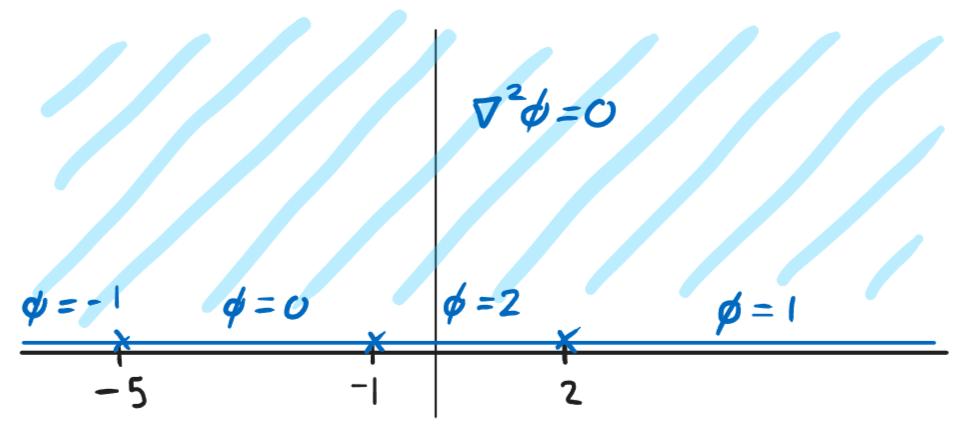
\includegraphics[width=0.8\textwidth]{Images/ComplexAnalysisPictures/ArgumentLaplacian.png}}\\
One trick to solve a problem like this is to choose a linear combination of functions of the form $\Arg(z-z_0)$ with a different point $z_0$ for every place where the boundary condition changes along the x-axis.
\begin{align*}
    &\phi=A_1\Arg(z+5)+A_2\Arg(z+1)+A_3\Arg(z-2)+A_4\\
    &\phi(x>2,0)=A_4=1\\
    &\phi(-1<x<2,0)=\pi A_3+1=2\Ra A_3=\frac{1}{\pi}\\
    &\phi(-5<x<-1,0)=\pi A_2+1+1=0\Ra A_2=-\frac{2}{\pi}\\
    &\phi(x<-5,0)=\pi A_1-2+2=-1\Ra A_1=-\frac{1}{\pi}\\
    &\phi(x,y)=-\frac{1}{\pi}\Arg(z+5)-\frac{2}{\pi}\Arg(z+1)+\frac{1}{\pi}\Arg(z-2)+1
\end{align*}
We can also apply these techniques to other types of boundary conditions in some cases.\\
Ex5: Given $\nabla^2\phi=0$ in the circular region $\brcurly{z: 1\leq |z|\leq 2}$ with the boundary conditions $\phi=1$ for $|z|=1$ and $\pdx[\phi]{r}=2$ for $|z|=2$, find $\phi(x,y)$
\begin{align*}
    &\phi=A\ln r+B\\
    &\phi(1)=B=1\\
    &\pdx[\phi(2)]{r}=\frac{A}{2}=2\Ra A=4\\
    &\phi=4\ln r+1\\
    &\phi(x,y)=4\ln\sqrt{x^2+y^2}+1
\end{align*}
If we have a region that has a semicircle in it we can use the Joukowski mapping to transform it into a region that is easier to work with.\\
\centerline{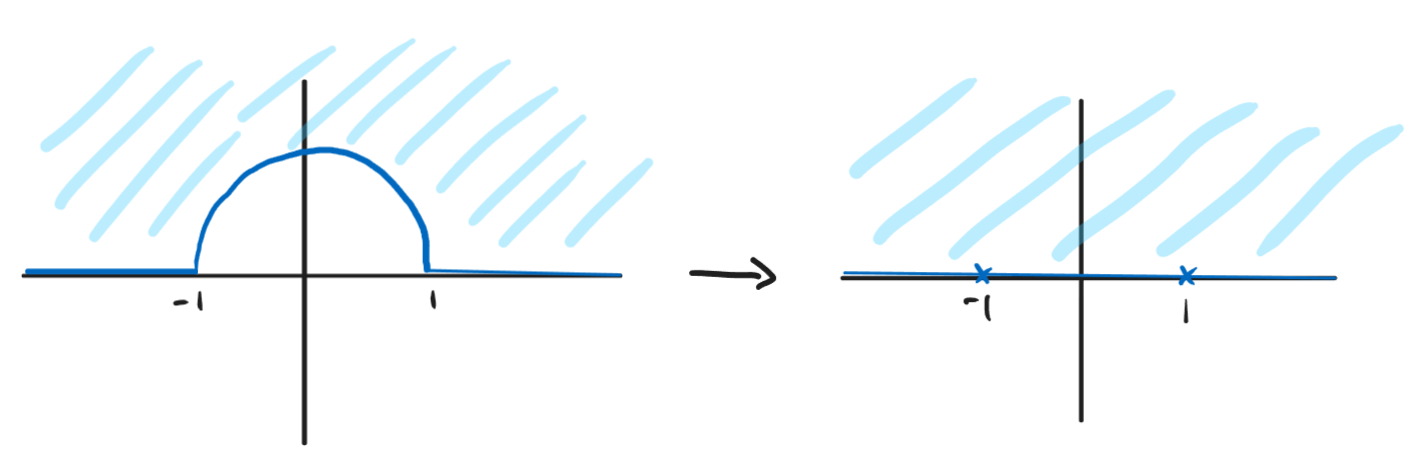
\includegraphics[width=0.95\textwidth]{Images/ComplexAnalysisPictures/JoukowskiMap.png}}\\
Ex6: Given $\nabla^2\phi=0$ in the upper region of the plane described by $\brcurly{y>0\wedge x^2+y^2>9}$ with the boundary conditions $\phi=-1$ for $x<3$, $\phi=0$ for $x^2+y^2=9$, and $\phi=2$ for $x>3$, find $\phi(x,y)$.
\begin{align*}
    &\eqnsystem{\phi(x,0)=-1 & x<-3\\ \phi(x,y)=0 & x^2+y^2=9\\ \phi(x,0)=2 & x>3}\\
    &w=\frac{1}{2}\brround{\frac{z}{3}+\frac{3}{z}}=u+iv\\
    &\Phi=A_1\Arg(w+1)+A_2\Arg(w-1)+A_3\\
    &\Phi(u>1,v)=A_3=2\\
    &\Phi(-1<u<1,v)=\pi A_2+2=0\Ra A_2=-\frac{2}{\pi}\\
    &\Phi(u<-1,v)=\pi A_1-2+2=-1\Ra A_1=-\frac{1}{\pi}\\
    &\Phi=-\frac{1}{\pi}\Arg(w+1)-\frac{2}{\pi}\Arg(w-1)+2\\
    &\phi(z)=-\frac{1}{\pi}\Arg\brround{\frac{1}{2}\brround{\frac{z}{3}+\frac{3}{z}}+1}-\frac{2}{\pi}\Arg\brround{\frac{1}{2}\brround{\frac{z}{3}+\frac{3}{z}}-1}+2
\end{align*}
In the case that we have a semicircle not of radius 1 we can apply a scaling before the Joukowski mapping to get the correct radius.\\
\centerline{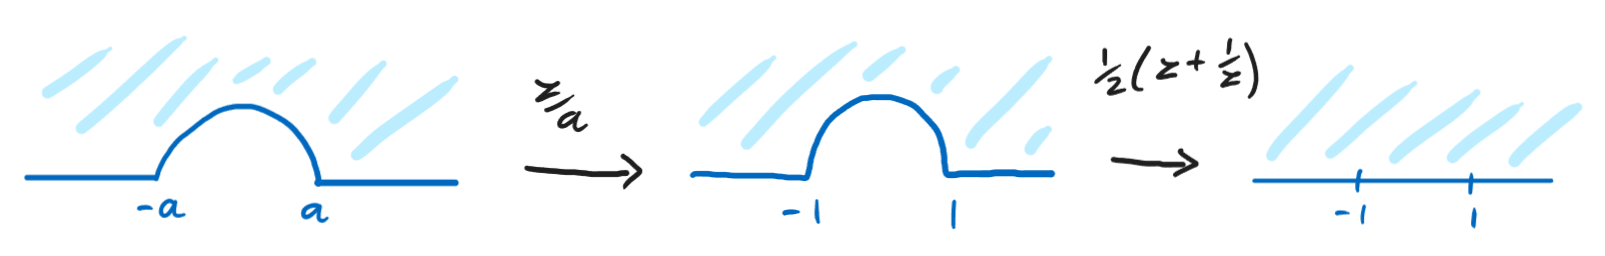
\includegraphics[width=0.95\textwidth]{Images/ComplexAnalysisPictures/JoukowskiShift.png}}
\[w=\frac{1}{2}\brround{\frac{z}{a}+\frac{a}{z}}\]

\subsubsection{Sinusoidal Functions}
If we recall Euler's formula $e^{ix}=\cos x+i\sin x$ we can use with complex numbers to get the following identities for complex sinusoidals:
\begin{itemize}
    \item $\sin z=\frac{e^{iz}-e^{-iz}}{2i}$
    \item $\cos z=\frac{e^{iz}+e^{-iz}}{2}$
    \item $\sinh z=\frac{e^z-e^{-z}}{2}$
    \item $\cosh z=\frac{e^z+e^{-z}}{2}$
    \item $\cos z=\sin\brround{\tfrac{\pi}{2}-z}$
    \item $\sinh z=-i\sin\brround{iz}$
    \item $\cosh z=\cos\brround{iz}=\sin\brround{\tfrac{\pi}{2}-iz}$
    \item $\ddx{z}\sin z=\cos z$
    \item $\ddx{z}\cos z=-\sin z$
    \item $\cos^2z+\sin^2z=1$
    \item $\ddx{z}\sinh z=\cosh z$
    \item $\ddx{z}\cosh z=\sinh z$
    \item $\cosh^2z-\sinh^2z=1$
\end{itemize}
The most notable difference between the real and complex versions of these functions is that $|\sin z|\not\leq1$. We will see cases of this soon but it is easy to see once we write out the real and imaginary components of $\sin z$.
\begin{align*}
    &\sin z=\sin(x+iy)=\frac{e^{i(x+iy)-e^{-i(x+iy)}}}{2i}=\frac{e^{-y}e^{ix}-e^ye^{-ix}}{2i}\\
    &\sin z = \frac{e^{-y}\brround{\cos x+i\sin x}-e^y\brround{\cos x-i\sin x}}{2i}=\frac{e^{-y}-e^y}{2}\cos x+\frac{e^{-y}+e^y}{2i}\sin x\\
    &\sin z = \sin x\cosh y+i\cos x\sinh y
\end{align*}
Ex: Find all solutions to $\sin z=4i$
\begin{align*}
    &\sin(z)=4i=\sin x\cosh y+i\cos x\sinh y\\
    &\sin x\cosh y=0\Ra \sin x=0\Ra x=n\pi\\
    &\text{Case 1: }n=2k:\ \cos x=1\\
    &4=\cos(2k\pi)\sinh(y)=\sinh y\\
    &\text{Case 2: }n=2k+1:\ \cos x=-1\\
    &4=\cos((2k+1)\pi)\sinh y=-\sinh y\\
    &\sinh y=\frac{e^{y}-e^{-y}}{2}\\
    &2\sinh y=e^y-e^{-y}\\
    &e^{2y}-2\sinh y e^{y}-1=0\\
    &e^y=\frac{2\sinh y\pm\sqrt{4\sinh^2y+4}}{2}=\sinh y\pm \sqrt{\sinh^2y+1}\\
    &n=2k:\\
    &y=\ln\brround{4\pm\sqrt{17}}=\ln\brround{4+\sqrt{17}}\\
    &n=2k+1:\\
    &y=\ln\brround{-4\pm\sqrt{17}}=\ln\brround{\sqrt{17}-4}\\
    &z=\brcurly{(x,y)\Bigg\vert\brround{2k\pi,\ln\brround{4+\sqrt{17}}},\brround{(2k+1)\pi,\ln\brround{\sqrt{17}-4},k\in\Z}}
\end{align*}
Ex2: Find all solutions to $\cos z=0$
\begin{align*}
    &\cos(z^4)=0\\
    &z^4=\pi n+\frac{\pi}{2}=\brround{\pi n+\frac{\pi}{2}}e^{2\pi il}\\
    &z=\brround{\pi n+\frac{\pi}{2}}^{1/4}e^{i\frac{\pi l}{2}},\ l=\brcurly{0,1,2,3},\ n\in\Z
\end{align*}

\textbf{Mapping properties of $\sin z$}\\
$\sin z$ will map the box $-\frac{\pi}{2}\leq x\leq\frac{\pi}{2},\ 0\leq y<\infty$ to the half plane $v>0$.\\
\centerline{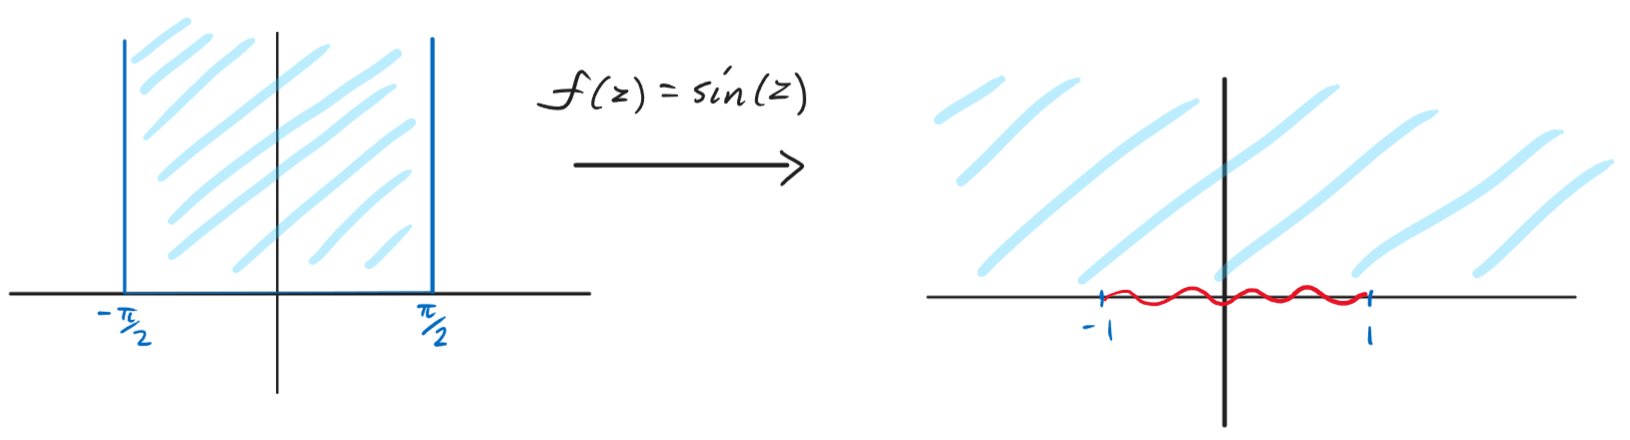
\includegraphics[width=0.95\textwidth]{Images/ComplexAnalysisPictures/SinMapping.png}}
Ex: Find the mapping of $\sin z$ on $S=\brcurly{-\frac{\pi}{2}<x<\frac{\pi}{2},0<y<1}$
\begin{align*}
    &u=\sin x\cosh y\\
    &\sin x\in(-1,1)\\
    &\cosh y \in (0,\cosh(1))\\
    &u\in (-\cosh(1),\cosh(1))\\
    &v=\cos x\sinh y\\
    &\cos x\in (0,1]\\
    &\sinh y\in (0,\sinh(1))\\
    &v\in(0,\sinh(1))\\
    &S'=\brcurly{(u,v)|-\cosh(1)<u<\cosh(1),0<v<\sinh(1)}
\end{align*}
If the box is offcenter we can also apply a composition of mappings to shift it into the usual form.\\
\centerline{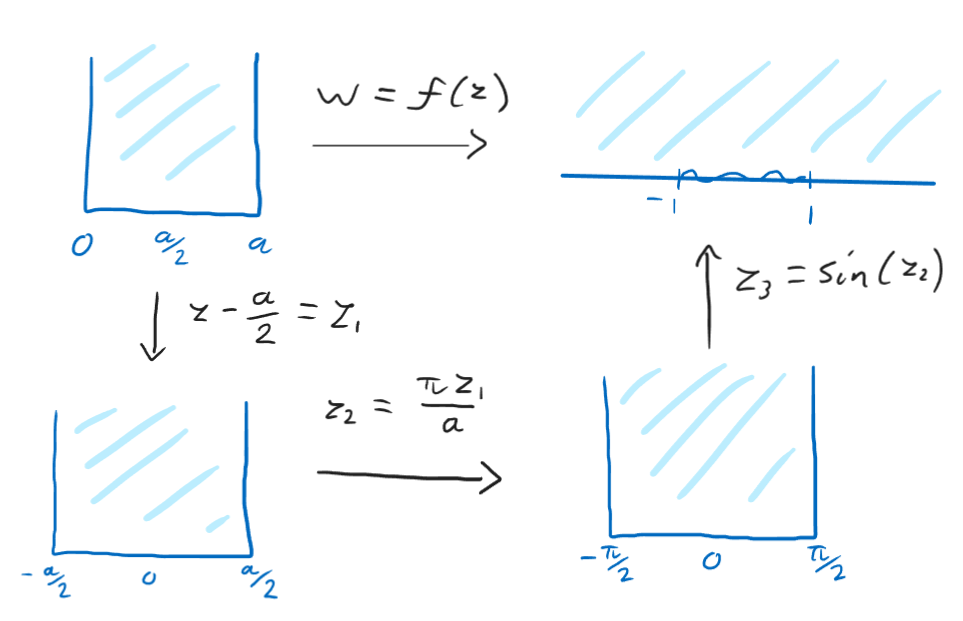
\includegraphics[width=0.85\textwidth]{Images/ComplexAnalysisPictures/TranslateSinMap.png}}
Ex2: Find the mapping of $\sin z$ on $S=\brcurly{-1<x<1,y>0}$
\begin{align*}
    &u=\sin x\cosh y\\
    &\sin x \in(-\sin(1),\sin(1))\\
    &\cosh y\in (1,\infty)\\
    &u\in \R\\
    &v=\cos x\sinh y\\
    &\cos x\in (\cos(1),1]\\
    &\sinh y \in (0,\infty)\\
    &v\in (0,\infty)\\
    &S'=\brcurly{(u,v)|v>0}
\end{align*}
Ex3: Solve the Laplace equation $\nabla^2u=0$ in the region $S=\brcurly{0\leq x\leq 2,0\leq y<\infty}$ with boundary conditions $\phi=0$ on $x=0$ and $\phi=1$ on $y=0$ and $\phi=-2$ on $x=2$.
\begin{align*}
    &\text{Map to the half plane using }w=\sin\brround{\frac{\pi}{2}(z-1)}\\
    &\phi(z)=\Phi(w)=A_1\Arg(w+1)+A_2\Arg(w-1)+A_3\\
    &u>1:\ \Phi=-2=A_3\\
    &-1<u<1:\ \Phi=1=A_2\pi-2\Ra A_2=\frac{3}{\pi}\\
    &u<-1:\ \Phi=0=A_1\pi+\frac{3}{\pi}\pi-2\Ra A_1=-\frac{1}{\pi}\\
    &\phi(z)=-\frac{1}{\pi}\Arg\brround{\sin\brround{\frac{\pi}{2}(z-1)}+1}+\frac{3}{\pi}\Arg\brround{\sin\brround{\frac{\pi}{2}(z-1)}-1}-2
\end{align*}

\subsubsection{Logarithmic Functions}
$\log z$ is defined as the inverse of $e^z$.
\begin{align*}
    &e^w=z\Ra w=\log z\\
    &w=u+iv\\
    &z=re^{i\Arg(z)}\\
    &e^ue^{iv}=re^{i\Arg(z)}\\
    &e^u=r\Ra u=\ln r\\
    &e^{iv}=e^{i\Arg(z)}\Ra v=\Arg(z)+2k\pi\\
    &\log(z)=w=\ln r+i(\Arg z+2k\pi),\ k\in\Z\\
    &\log(z)=\brcurly{w|e^w=z}=\ln r+i(\Arg z+2k\pi)=\ln r+i\arg z\\
    &\Log(z)=\ln r+i\Arg z
\end{align*}
Note that $\log(z)=\ln r+i\arg z$ is a multi-valued function and $\Log(z)=\ln r+i\Arg z$ is the principal value of $\log z$.\\
Ex: Find all values for $\log 2$ and $\Log 2$.
\begin{align*}
    &z=2=2e^{i0}\\
    &\log 2=\ln 2+i(0+2k\pi)=\ln 2+2k\pi i,\ k\in\Z\\
    &\Log 2=\ln 2+i(0)=\ln 2
\end{align*}
Ex2: Find all values for $\log(-1-\sqrt{3}i)$ and $\Log(-1-\sqrt{3}i)$.
\begin{align*}
    &z=-1-\sqrt{3}i=2e^{i\frac{2\pi}{3}}\\
    &\log(-1-\sqrt{3}i)=\ln 2+i\brround{-\frac{2\pi}{3}+2k\pi},\ k\in\Z\\
    &\Log(-1-\sqrt{3}i)=\ln 2+i\brround{-\frac{2\pi}{3}}
\end{align*}
Ex3: Find all values for $\log(e^{1+5i})$ and $\Log(e^{1+5i})$.
\begin{align*}
    &z=e^{1+5i}=ee^{5i}=ee^{i(5+2k\pi)}\\
    &5+2k\pi\in(-\pi,\pi]\Ra k=-1\\
    &\Arg(e^{1+5i})=5-2\pi\\
    &\log(e^{1+5i})=\ln e+i(5-2\pi+2k\pi)=1+i(5-2\pi+2k\pi),\ k\in\Z\\
    &\Log(e^{1+5i})=\ln e+i(5-2\pi)=1+i(5-2\pi)
\end{align*}
Ex4: Find all values for $\log(-i)$ and $\Log(-i)$.
\begin{align*}
    &-i=e^{-i\frac{\pi}{2}}\\
    &\arg(-i)=-\frac{\pi}{2}+2\pi k\\
    &\log(-i)=-i\frac{\pi}{2}+i2\pi k\\
    &\Log(-i)=-i\frac{\pi}{2}
\end{align*}

Properties of $\log z$ and $\Log z$:
\begin{itemize}
    \item $\log(z_1z_2)=\log z_1+\log z_2$\\
    $\Log(z_1z_2)\neq\Log z_1+\Log z_2$ (same as why $\Arg(z_1z_2)\neq\Arg(z_1)+\Arg(z_2)$)
    \item $e^{\log z}=z$ and $e^{\Log z}=z$\\
    but $\log(e^z)\neq z$ and $\Log(e^z)\neq z$\\
    Ex: $z=0$: $\log(e^0)=\log(1)=\ln1+i(0+2k\pi)=i2k\pi\neq0$\\
    $\Log(e^{5i})=i(5-2\pi)\neq 5i$\\
    rather $z\in\log(e^z)$
    \item $\log z^n\neq n\log z$
    \begin{align*}
        &z=1,\ n=2:\ \log z^2=\log 1=i2k\pi\\
        &2\log z=2\log 1=2i(2k')\pi
    \end{align*}
    but $\log z^\frac{1}{n}=\frac{1}{n}\log z$
    \item $\Log z$ is analytic in $\C\backslash(-\infty,0]$\\
    \centerline{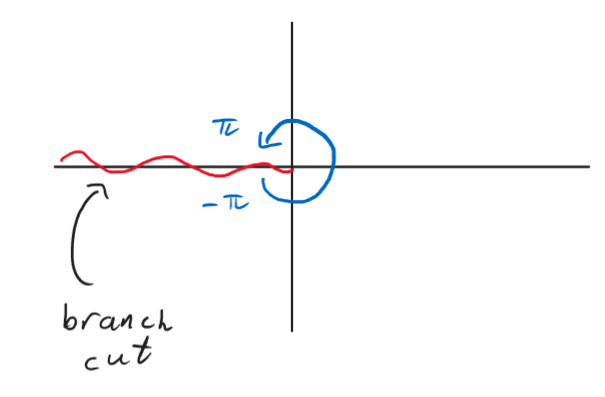
\includegraphics[width=0.6\textwidth]{Images/ComplexAnalysisPictures/BranchCut.png}}
    $\Log z=\ln|z|+i\Arg z,\ -\pi<\Arg z<\pi$
\end{itemize}
Ex: Find all solutions to $e^z=-1-i$
\begin{align*}
    &z=\log(-1-i)\\
    &-1-i=\sqrt{2}e^{-i\frac{3\pi}{4}}\\
    &z=\frac{1}{2}\ln(2)-i\frac{3\pi}{4}+i2\pi k
\end{align*}
Ex2: Find the principal value of $(1+i)^i=e^{i\Log(1+i)}$
\begin{align*}
    &1+i=\sqrt{2}e^{i\frac{\pi}{4}}\\
    &\Log(1+i)=\frac{1}{2}\ln(2)+i\frac{\pi}{4}\\
    &(1+i)^i=e^{-\frac{\pi}{4}+i\frac{1}{2}\ln(2)}
\end{align*}
Ex3: Find the principle value of $z^i=1+i$
\begin{align*}
    &1+i=\sqrt{2}e^{i\frac{\pi}{4}+i2\pi k}=e^{\ln(\sqrt{2})+i\frac{\pi}{4}+i2\pi k}\\
    &z=(1+i)^{1/i}=(1+i)^{-i}=e^{\frac{\pi}{4}+2\pi k}e^{-i\ln(\sqrt{2})}\\
    &z=e^{\frac{\pi}{4}}e^{-i\frac{1}{2}\ln(2)}
\end{align*}
Ex4: Find the principal value of $i^i$.
\begin{align*}
    &i^i=(e^{i\frac{\pi}{2}+i2\pi k})^i=e^{-\frac{\pi}{2}-2\pi k}=e^{-\frac{\pi}{2}}
\end{align*}
Ex5: Find all solutions to $\Log(z^2-1)=\frac{i\pi}{2}$
\begin{align*}
    &z^2-1=e^{i\frac{\pi}{2}}=i\\
    &z^2=i+1=\sqrt{2}e^{i\frac{\pi}{4}+i2\pi k}\\
    &z=2^{1/4}e^{i\frac{\pi}{8}+i\pi k}
\end{align*}
Ex6: Find all solutions to $e^{2z}+e^z+1=0$
\begin{align*}
    &e^z=\frac{-1\pm\sqrt{1-4}}{2}=-\frac{1}{2}\pm i\frac{\sqrt{3}}{2}\\
    &e^z=e^{i\pi\pm i\frac{\pi}{3}+i2\pi k}\\
    &z=i\pi\pm i\frac{\pi}{3}+i2\pi k\\
    &z=\pm i\frac{2\pi}{3}+i2\pi k
\end{align*}

\textit{Derivative of $\log z$ and $\Log z$}
\begin{align*}
    &(\Log z)'=\frac{1}{z}\\
    &\Log z=\ln\sqrt{x^2+y^2}+i\Arg z=u+iv\\
    &(\Log z)'=u_x+iv_x\\
    &\Log z=\ln|z|+i\varphi,\ -\pi<\varphi<\pi
\end{align*}

\subsubsection{Branch Cuts}
There are many different analytic functions for $\log z$ depending on the branch cut we choose. For example we can choose:
\begin{align*}
    &\Log z=\ln r +i\varphi,\ -\pi<\varphi<\pi,\ \C\backslash(-\infty,0]\\
    &\log z=\ln r +i\varphi,\ 0<\varphi<2\pi,\ \C\backslash[0,\infty)\\
    &\log z=\ln r +i\varphi,\ -\frac{\pi}{2}<\varphi<\frac{5\pi}{2},\ \C\backslash i[0,\infty)
\end{align*}
Ex: Specify a branch cut for $\log z$ such that it is analytic at $z=-1,-i,1$
\[\log z=\ln r+i\varphi,\ \frac{\pi}{2}<\varphi<\frac{5\pi}{2}\]

The reason we have branch cuts is so that we can define a single-valued analytic function. This is important for functions such as $\sqrt{z}$ and $\log z$ as one input can correspond to multiple outputs. For example, $\sqrt{1}=1$ and $\sqrt{1}=-1$. This is why we need to specify a branch cut for $\sqrt{z}$ and $\log z$.
Ex: Construct $f(z)=z^{1/2}$ such that it is analytic in $\C\backslash(-\infty,0]$ and $f(1)=-1$.
\begin{align*}
    &z^\frac{1}{2}=e^{\frac{1}{2}\log z}=e^{\frac{1}{2}\ln r+i\frac{1}{2}\varphi}=r^\frac{1}{2}e^{i\frac{\varphi}{2}},\ -\pi<\varphi<\pi\\
    &f(1)=r^\frac{1}{2}e^{i\frac{\varphi}{2}}=1e^{i0}=1\\
    &z^\frac{1}{2}=r^\frac{1}{2}e^{i\frac{\varphi}{2}},\ \pi<\varphi<3\pi\\
    &\to f(1)=1^\frac{1}{2}e^{\frac{2\pi}{2}}=-1
\end{align*}
Ex2: Find all solutions to $z^{1/2}+1-i=0$ where $z^{1/2}$ is the principal branch of $z^{1/2}$.
\begin{align*}
    &z^{1/2}=|z|^{1/2}e^{i\frac{\varphi}{2}}=i-1=\sqrt{2}e^{i\frac{3\pi}{4}+i2\pi k}\\
    &|z|e^{i\varphi}=2e^{i\frac{3\pi}{2}+i4\pi k}\\
    &|z|=2\\
    &\varphi=\frac{3\pi}{2}+4\pi k\not\in(-\pi,\pi]\\
    &\therefore\text{ no solutions}
\end{align*}
Ex3: Find all solutions to $z^{1/2}+1-i=0$
\begin{align*}
    &\\
    &z^{1/2}=|z|^{1/2}e^{i\frac{\varphi}{2}+i\pi k_1}i-1=\sqrt{2}e^{i\frac{3\pi}{4}+i2\pi k_2}\\
    &|z|e^{i\varphi+i2\pi k_1}=2e^{i\frac{3\pi}{2}+i4\pi k_2}\\
    &|z|=2\\
    &\varphi+2\pi k_1=\frac{3\pi}{2}+4\pi k_2\\
    &\varphi=\frac{3\pi}{2}+2\pi k_3\\
    &z=2e^{-i\frac{\pi}{2}}=-2i
\end{align*}
Ex4: Find where $\Log(1+z^2)$ is analytic
\begin{align*}
    &w=1+z^2\\
    &\text{not analytic on }\Re(w)\leq0\ \wedge \Im(w)=0\\
    &x^2-y^2+1\leq0\\
    &2xy=0\Ra x=0 \vee y=0\\
    &y=0:\ x^2+1\leq 0\Ra \nexists x\in\R\text{ s.t. }x^2\leq-1\\
    &x=0:\ y^2\geq 1\Ra |y|\geq 1
\end{align*}
Analytic on the domain
\[ \C\backslash\brcurly{(x,y):x=0,|y|\geq1} \]
Ex5: Find where $\Log\bfrac{1-z}{1+z}$ is analytic
\begin{align*}
    &w=\frac{1-z}{1+z}\\
    &\text{not analytic on }\Re(w)\leq 0\ \wedge\Im(w)=0\\
    &w=\frac{(1-z)(1+\overline{z})}{(1+z)(1+\overline{z})}=\frac{1-|z|^2-z+\overline{z}}{1+|z|^2+z+\overline{z}}=\frac{1-x^2-y^2-2iy}{1+x^2+y^2+2x}\\
    &y=0\\
    &\frac{1-x^2}{1+x^2+2x}\leq0\Ra 1\leq x^2\Ra |x|\geq 1
\end{align*}
Analytic on
\[ \C\backslash\brcurly{(x,y):y=0,|x|\geq1} \]
Ex6: Find a branch cut for $f(z)=\sqrt{z(z-1)}$ such that it is analytic for $\brcurly{(x,y)|y=0,x<0}$ such that $f(2)=\sqrt{2}$
\begin{align*}
    &\sqrt{z(z-1)}=|z|^{1/2}e^{i\frac{\varphi_1}{2}}|z-1|^{1/2}e^{i\frac{\varphi_2}{2}}=(|z||z-1|)^{1/2}e^{i\frac{\varphi_1+\varphi_2}{2}}\\
    &\varphi_1\in(-\pi,\pi),\ \varphi_2\in(-\pi,\pi)\\
    &\lim_{\varphi_1\to\pi}\lim_{\varphi_2\to\pi}e^{i\frac{\varphi_1+\varphi_2}{2}}=e^{\pi i}\\
    &\lim_{\varphi_1\to-\pi}\lim_{\varphi_2\to-\pi}e^{i\frac{\varphi_1+\varphi_2}{2}}=e^{-\pi i}=e^{\pi i}\\
    &\therefore \text{ continuous for }\brcurly{(x,y)|y=0,x<0}\\
    &z=2:\ \varphi_1=0,\ \varphi_2=0\Ra \sqrt{z(z-1)}=\sqrt{2}
\end{align*}
Ex7: Find a branch cut for $f(z)=\sqrt{z(z-1)}$ such that it is analytic for $\brcurly{(x,y)|y=0,x<0}$ such that $f(2)=-\sqrt{2}$
\begin{align*}
    &\sqrt{z(z-1)}=|z|^{1/2}e^{i\frac{\varphi_1}{2}}|z-1|^{1/2}e^{i\frac{\varphi_2}{2}}=(|z||z-1|)^{1/2}e^{i\frac{\varphi_1+\varphi_2}{2}}\\
    &\varphi_1\in(-\pi,\pi),\ \varphi_2\in(-3\pi,-\pi)\\
    &\lim_{\varphi_1\to\pi}\lim_{\varphi_2\to-\pi}e^{i\frac{\varphi_1+\varphi_2}{2}}=e^{-2\pi i}\\
    &\lim_{\varphi_1\to-\pi}\lim_{\varphi_2\to-3\pi}e^{i\frac{\varphi_1+\varphi_2}{2}}=e^{0}=e^{-2\pi i}\\
    &\therefore \text{ continuous for }\brcurly{(x,y)|y=0,x<0}\\
    &z=2:\ \varphi_1=0,\ \varphi_2=-2\pi\Ra \sqrt{z(z-1)}=\sqrt{2}e^{-i\pi}=-\sqrt{2}
\end{align*}
Ex8: Find a branch cut for $f(z)=\log(z^2+2z+2)$ such that it is analytic for $\brcurly{(x,y)|x>-1}$ such that $\ddx{z}f(-1)=0$
\begin{align*}
    &\log(z^2+2z+2)\\
    &z=\frac{-2\pm\sqrt{4-8}}{2}=-1\pm i\\
    &\log(z^2+2z+2)=\ln(|z-z_1||z-z_2|)+i(\varphi_1+\varphi_2)\\
    &-\pi<\varphi_1<\pi,\ -\pi<\varphi_2<\pi\\
    &z=-1:\ \varphi_1=-\frac{\pi}{2},\ \varphi_2=\frac{\pi}{2}\\
    &\log(z^2+2z+2)\eval_{z=-1}=0+i\brround{-\frac{\pi}{2}+\frac{\pi}{2}}=0\\
    &\ddx{z}\log(z^2+2z+2)\eval_{z=-1}=\frac{2z+2}{z^2+2z+2}\eval_{z=-1}=0
\end{align*}